\documentclass[
  bibliography=totoc,     % Literatur im Inhaltsverzeichnis
  captions=tableheading,  % Tabellenüberschriften
  titlepage=firstiscover, % Titelseite ist Deckblatt
]{scrartcl}

% Vektoren
\usepackage{esvect}


% Paket float verbessern
\usepackage{scrhack}

% Warnung, falls nochmal kompiliert werden muss
\usepackage[aux]{rerunfilecheck}

% unverzichtbare Mathe-Befehle
\usepackage{amsmath}
% viele Mathe-Symbole
\usepackage{amssymb}
% Erweiterungen für amsmath
\usepackage{mathtools}

% Fonteinstellungen
\usepackage{fontspec}
% Latin Modern Fonts werden automatisch geladen
% Alternativ zum Beispiel:
%\setromanfont{Libertinus Serif}
%\setsansfont{Libertinus Sans}
%\setmonofont{Libertinus Mono}

% Wenn man andere Schriftarten gesetzt hat,
% sollte man das Seiten-Layout neu berechnen lassen
\recalctypearea{}

% deutsche Spracheinstellungen
\usepackage{polyglossia}
\setmainlanguage{german}

% Blindtext
\usepackage{blindtext}

\usepackage[
  math-style=ISO,    % ┐
  bold-style=ISO,    % │
  sans-style=italic, % │ ISO-Standard folgen
  nabla=upright,     % │
  partial=upright,   % ┘
  warnings-off={           % ┐
    mathtools-colon,       % │ unnötige Warnungen ausschalten
    mathtools-overbracket, % │
  },                       % ┘
]{unicode-math}

% traditionelle Fonts für Mathematik
\setmathfont{Latin Modern Math}
% Alternativ zum Beispiel:
%\setmathfont{Libertinus Math}

\setmathfont{XITS Math}[range={scr, bfscr}]
\setmathfont{XITS Math}[range={cal, bfcal}, StylisticSet=1]

% Zahlen und Einheiten
\usepackage[
  locale=DE,                   % deutsche Einstellungen
  separate-uncertainty=true,   % immer Fehler mit \pm
  per-mode=symbol-or-fraction, % / in inline math, fraction in display math
]{siunitx}

% chemische Formeln
\usepackage[
  version=4,
  math-greek=default, % ┐ mit unicode-math zusammenarbeiten
  text-greek=default, % ┘
]{mhchem}

% richtige Anführungszeichen
\usepackage[autostyle]{csquotes}

% schöne Brüche im Text
\usepackage{xfrac}
\usepackage{nicefrac}

% Standardplatzierung für Floats einstellen
\usepackage{float}
\floatplacement{figure}{htbp}
\floatplacement{table}{htbp}

% Floats innerhalb einer Section halten
\usepackage[
  section, % Floats innerhalb der Section halten
  below,   % unterhalb der Section aber auf der selben Seite ist ok
]{placeins}

% Seite drehen für breite Tabellen: landscape Umgebung
\usepackage{pdflscape}

% Captions schöner machen.
\usepackage[
  labelfont=bf,        % Tabelle x: Abbildung y: ist jetzt fett
  font=small,          % Schrift etwas kleiner als Dokument
  width=0.9\textwidth, % maximale Breite einer Caption schmaler
]{caption}
% subfigure, subtable, subref
\usepackage{subcaption}

% Grafiken können eingebunden werden
\usepackage{graphicx}
% größere Variation von Dateinamen möglich
\usepackage{grffile}

% schöne Tabellen
\usepackage{booktabs}

% Verbesserungen am Schriftbild
\usepackage{microtype}

% Literaturverzeichnis
\usepackage[
  backend=biber,
]{biblatex}
% Quellendatenbank
\addbibresource{lit.bib}
\addbibresource{programme.bib}

% Hyperlinks im Dokument
\usepackage[
  unicode,        % Unicode in PDF-Attributen erlauben
  pdfusetitle,    % Titel, Autoren und Datum als PDF-Attribute
  pdfcreator={},  % ┐ PDF-Attribute säubern
  pdfproducer={}, % ┘
]{hyperref}
% erweiterte Bookmarks im PDF
\usepackage{bookmark}

% Trennung von Wörtern mit Strichen
\usepackage[shortcuts]{extdash}
%Erlaubt Einfügen von PDF-Dateien
\usepackage{pdfpages}
\author{%
  Lars Kolk\\%
  \href{mailto:lars.kolk@tu-dortmund.de}{lars.kolk@tu-dortmund.de}%
  \texorpdfstring{\and}{,}%
  Julia Sobolewski\\%
  \href{mailto:julia.sobolewski@tu-dortmund.de}{julia.sobolewski@tu-dortmund.de}%
  \texorpdfstring{\and}{,}%
  Jannine Salewski\\%
  \href{mailto:Jannine.salewski@tu-dortmund.de}{jannine.salewski@tu-dortmund.de}%
}
\publishers{TU Dortmund – Fakultät Physik}

\usepackage{longtable}
\usepackage{wrapfig}
\usepackage{ dsfont }
\usepackage{tcolorbox}
\subject{SMD-Abgabe}
\title{4. Übungsblatt}
\date{%
  Abgabe: 15.11.2018
}

\begin{document}
  \setlength{\parindent}{0em}
  \maketitle
  \thispagestyle{empty}
  \newpage
  %\tableofcontents
  %\newpage

  \newenvironment{console1}[1]
  {\begin{center}
  \begin{minipage}[t]{0.99\linewidth}
  \begin{tcolorbox}[colback=gray!5,colframe=black!40!black,title= Ausgabe des Programms: #1 ]
    }
    {
  \end{tcolorbox}
  \end{minipage}
  \end{center}
  }

\paragraph{Aufgabe 13}


\subparagraph{a) und b)}
Für die Teilaufgabe \textbf{b)} ergibt sich das in \ref{fig:13ab} zu sehende Histogramm.
\begin{figure}[H]
  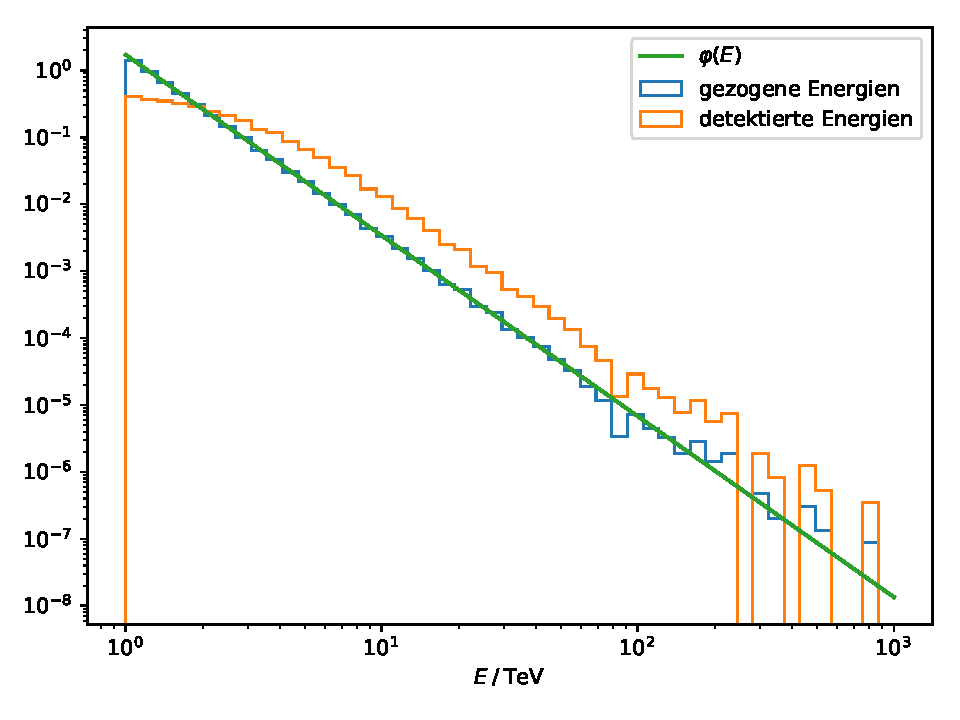
\includegraphics{Aufgabe13/b.pdf}
  \caption{Histogramm der gezogenen und detektiertenEnergien }
  \label{fig:13ab}
\end{figure}

\subparagraph{c) und d)}
 Mit den in \textit{c)} erzeugten, normalverteilten Hits folgt das in \ref{fig:13cd} zu sehende \textit{2D-Histogramm} für die gemessenden Ereignisse auf einem quadratischen Detektor.
 \begin{figure}[H]
   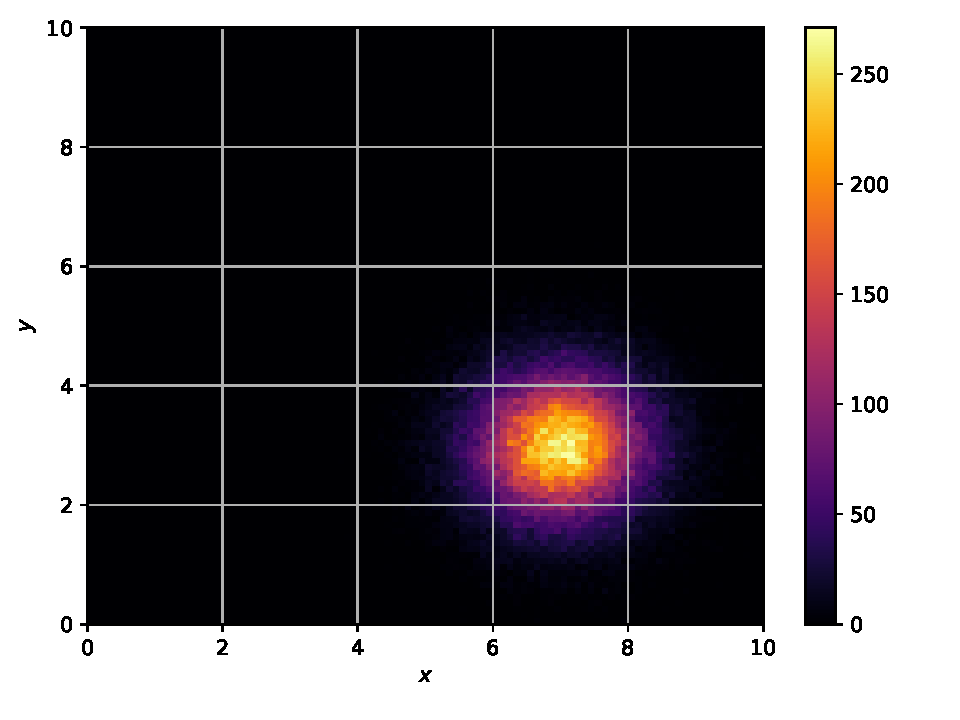
\includegraphics{Aufgabe13/d.pdf}
   \caption{Histogramm der gemessenen Ereignisse auf einem quadratischen Detektor }
   \label{fig:13cd}
 \end{figure}

 \subparagraph{e)}
 Für den Logarithmus der Anzahl der Hits folgt das in \ref{fig:13ehits} zu sehende \textit{Histogramm}.
 \begin{figure}[H]
   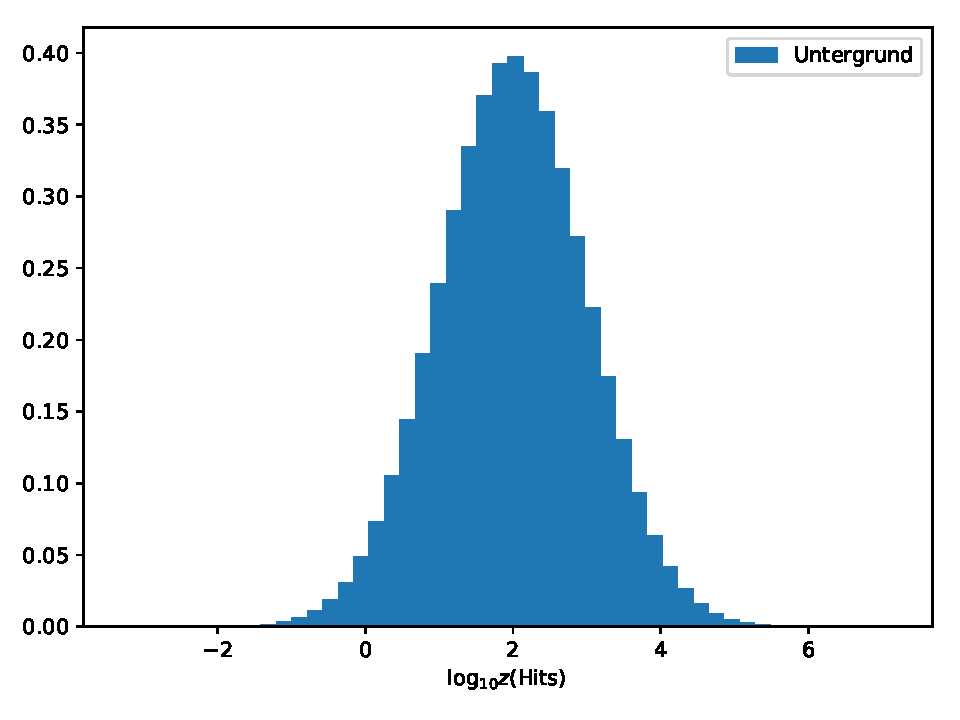
\includegraphics{Aufgabe13/e_hits.pdf}
   \caption{Histogramm für für Logarithmus der Anzahl der Hits}
   \label{fig:13ehits}
 \end{figure}
 Für die Orte der Untergrundereignisse folgt das in \ref{fig:13edetektor} zu sehende \textit{2D-Histogramm}.
 \begin{figure}[H]
   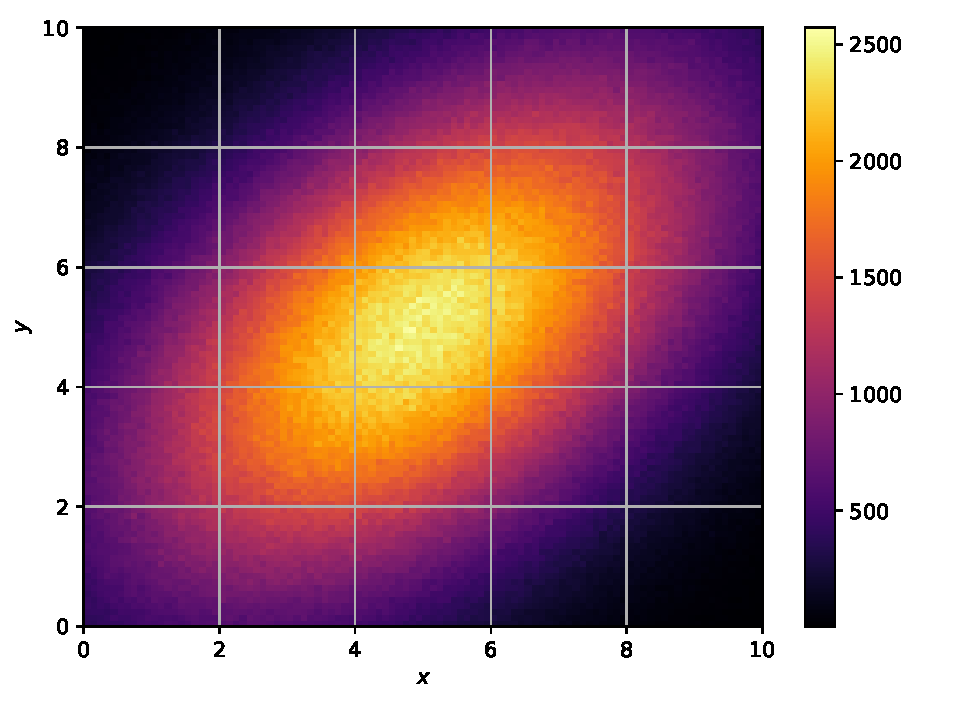
\includegraphics{Aufgabe13/e_detektor.pdf}
   \caption{Histogramm für für Logarithmus der Anzahl der Hits}
   \label{fig:13edetektor}
 \end{figure}

%\section{Aufgabe 12}
\subsection{a)}
Mittelwerte:
\begin{equation*}
  \vec{\mu}_0 = \begin{pmatrix}
                  -0,027\\
                   2,980\\
  \end{pmatrix}
\end{equation*}
\begin{equation*}
  \vec{\mu}_1 = \begin{pmatrix}
                   5,986\\
                   3,085\\
  \end{pmatrix}
\end{equation*}

\subsection{b)}
Kovarianzmatrizen:
\begin{equation*}
  V_0 = \begin{pmatrix}
                  12,209 &  8,158 \\
                  8,158  &  6,7223 \\
  \end{pmatrix}
\end{equation*}
\begin{equation*}
  V_1 = \begin{pmatrix}
                  12,352 &  7,411 \\
                  7,411 &  5,477 \\
  \end{pmatrix}
\end{equation*}

Kombinierte Kovaranzmatrix:
\begin{equation*}
  V_{\symup{0,1}} = \begin{pmatrix}
                  21,322 &  7,943 \\
                  7,943 &  6,103 \\
  \end{pmatrix}
\end{equation*}

\subsection{c)}
Zu Berechnung der Fisher-Diskriminante, müssen zunächst die Streumatrizen berechnet werden:
\begin{equation*}
  S_0 = \begin{pmatrix}
                  122077,077 & 81575,940 \\
                  81575,940 & 67221,910 \\
  \end{pmatrix}
\end{equation*}
\begin{equation*}
  S_1 = \begin{pmatrix}
                  123509.502 & 74100.151 \\
                  74100.151 & 54767.673 \\
  \end{pmatrix}
\end{equation*}

Daraus wird die Gesamtstreuung $S_W$ berechnet
\begin{equation*}
  S_W = S_0 + S_1= \begin{pmatrix}
                  245586,579 & 155676,091 \\
                  155676,091 & 121989,583 \\
  \end{pmatrix}
\end{equation*}
Die Fisher-Diskriminante lässt sich nun mit Hilfe der Formel
\begin{equation}
  \vec{\lambda} = S_W^{-1} (\vec{\mu_0} - \vec{\mu_1})
\end{equation}
berechnen:
\begin{equation*}
  \vec{\lambda} = \begin{pmatrix}
                  -0,0001253 \\
                  0,00015904 \\
  \end{pmatrix}
\end{equation*}
Diese lässt sich als Geradengleichung der Form $\vec{\lambda} = \lambda \cdot \vec{e}_{\lambda}$  darstellen:, mit
\begin{equation*}
  \lambda = 0,00020247
\end{equation*}
und
\begin{equation}
  \label{Einheitsvektor}
  \vec{e}_{\lambda} = \begin{pmatrix}
                  -0,619 \\
                  0,785 \\
  \end{pmatrix}
\end{equation}
Der Einheitsvektor \eqref{Einheitsvektor} lässt sich für die Projektion in den nächsten Aufgabenteilen verwenden.

\subsection{d)}
Zu Projektion der einzelnen Punkte auf die Gerade $\vec{\lambda}$ wird folgende Formel verwendet:
\begin{equation*}
  P_{\symup{\lambda}}(\vec{x}) = ( \vec{x} \cdot \vec{e}_{\lambda} ) \cdot \vec{e}_{\lambda}
\end{equation*}
wobei für die eindimensionale Verteilung nur der Betrag genommen wird, also nur $(\vec{x}\cdot \vec{e}_{\lambda})$.
Die eindimensionale Verteilung auf der Geraden ist in Abbildung \ref{abb:1} zu sehen.

\begin{figure}
  \centering
  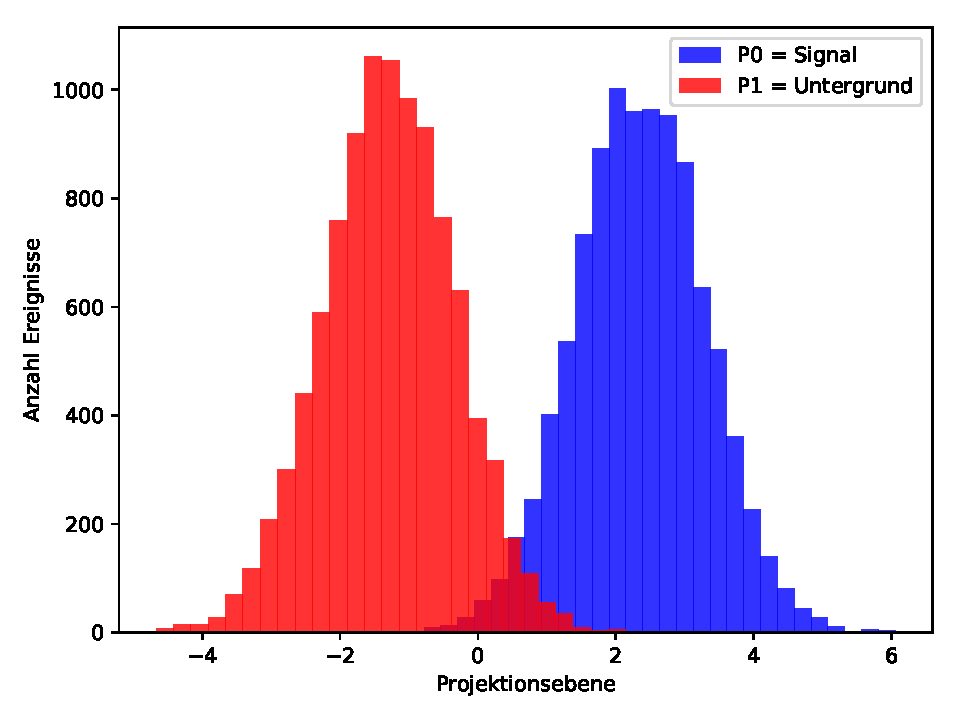
\includegraphics[scale=0.7]{Aufgabe12/Projektionen.pdf}
  \caption{Projektion auf die Gerade.}
  \label{abb:1}
\end{figure}

\subsection{e)}
Die Effizienz wird mit der Formel:
\begin{equation*}
  \symup{Effizienz} = \frac{t_p}{t_p + f_p}
\end{equation*}
berechnet und die Reinheit mir:
\begin{equation}
  \symup{Reinheit} = \frac{t_p}{t_p + f_n}
\end{equation}
Die Effizienz und die Reinheit in Abhängigkeit der Cut-Stelle $\lambda_{\symup{cut}}$ ist in Abbildung
\ref{abb:2} dargestellt.
\begin{figure}
  \centering
  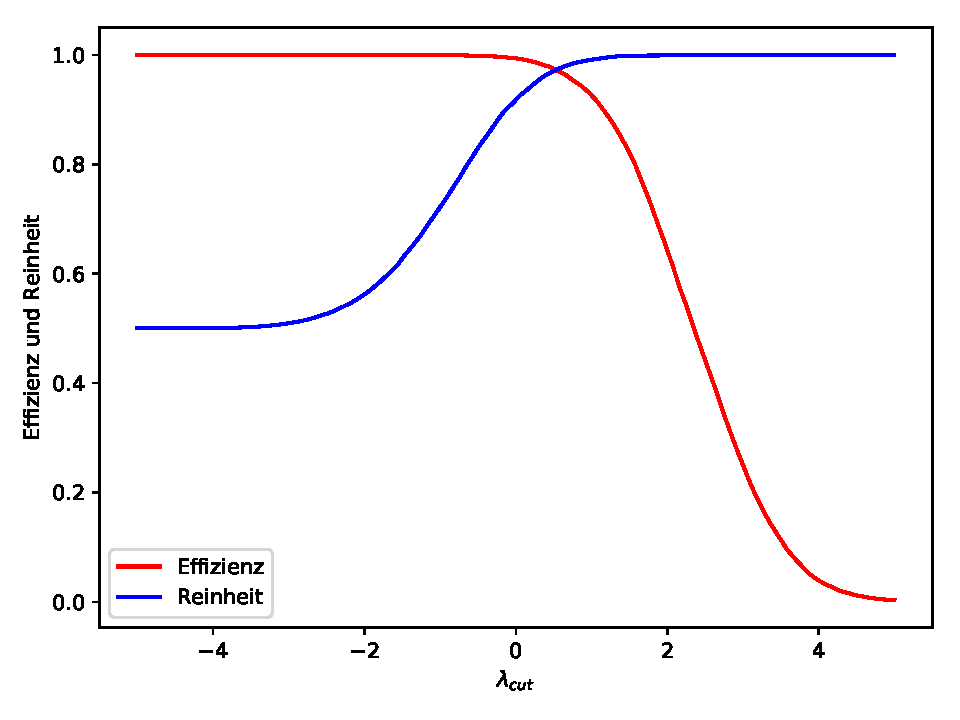
\includegraphics[scale=0.7]{Aufgabe12/EffizienzReinheit.pdf}
  \caption{Effizienz und Reinheit in Abhängigkeit der Cut-Stelle.}
  \label{abb:2}
\end{figure}

\subsection{f)}
Das Verhältnis zwischen Signal und Untergrund in Abhängigkeit von $\lambda_{\symup{cut}}$
ist in Abbildung \ref{abb:3} zu sehen. Der Maximalwert liegt hier bei
\begin{equation*}
  \lambda_{\symup{cut,Verhältnis}} \approx 2,17
\end{equation*}
\begin{figure}
  \centering
  \includegraphics[scale=0.7]{Aufgabe12/Verhältnis.pdf}
  \caption{Verhältnis S/B in Abhängigkeit der Cut-Stelle.}
  \label{abb:3}
\end{figure}

\subsection{g)}
Die Signifikanz $\frac{S}{\sqrt{S+B}} $ in Abhängigkeit von $\lambda_{\symup{cut}}$ ist in Abbildung
\ref{abb:4} dargestellt.
Der Maximalwert liegt hier bei:
\begin{equation*}
  \lambda_{\symup{cut, Signifikanz}} \approx 0,45
\end{equation*}
\begin{figure}
  \centering
  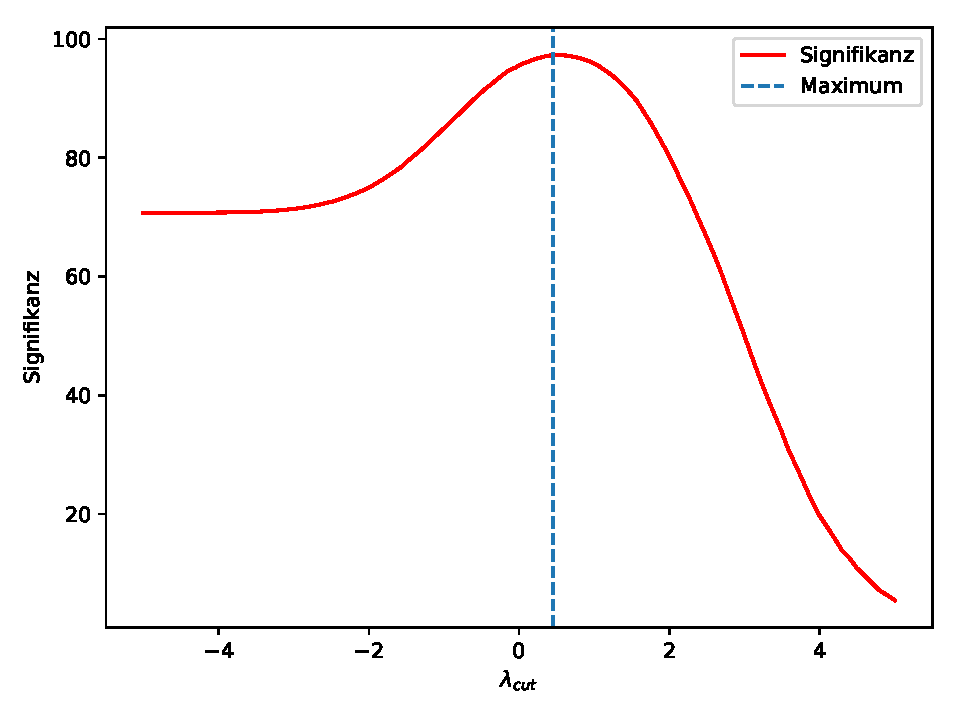
\includegraphics[scale=0.7]{Aufgabe12/Signifikanz.pdf}
  \caption{Signifikanz in Abhängigkeit der Cut-Stelle.}
  \label{abb:4}
\end{figure}

\subsection{f)}
Das ganze soll nun mit einem anderen Signal erneut untersucht werden:

Mittelwert:
\begin{equation*}
  \vec{\mu}_2 = \begin{pmatrix}
                  -0,0958\\
                   2,8788\\
  \end{pmatrix}
\end{equation*}

Kovarianzmatrix:
\begin{equation*}
  V_2 = \begin{pmatrix}
                  12,236 &  8,160 \\
                  8,160 &  6,758 \\
  \end{pmatrix}
\end{equation*}

Kombinierte Kovaranzmatrix:
\begin{equation*}
  V_{\symup{2,1}} = \begin{pmatrix}
                  15,398 &  7,582 \\
                  7,582 &  5,597 \\
  \end{pmatrix}
\end{equation*}

Streumatrix:
\begin{equation*}
  S_2 = \begin{pmatrix}
                  12223,886 & 81252,338 \\
                  81252,338 & 6751,132 \\
  \end{pmatrix}
\end{equation*}

Gesamtstreuung:
\begin{equation*}
  S_{W2} = \begin{pmatrix}
                  135733,388 & 82252,489 \\
                  82252,489 & 61519,105 \\
  \end{pmatrix}
\end{equation*}

Fisher-Diskriminante:
\begin{equation*}
  \vec{\lambda}_2 = \begin{pmatrix}
                  -0,000254 \\
                  0,000298 \\
  \end{pmatrix}
  = 0,374 \cdot 10^{-3} \begin{pmatrix}
                  -0,603 \\
                  0,797 \\
  \end{pmatrix}
  = \lambda_2 \cdot \vec{e}_{\lambda2}
\end{equation*}

Die eindimensionale Verteilung ist in Abbildung \ref{abb:5} dargestellt.

\begin{figure}
  \centering
  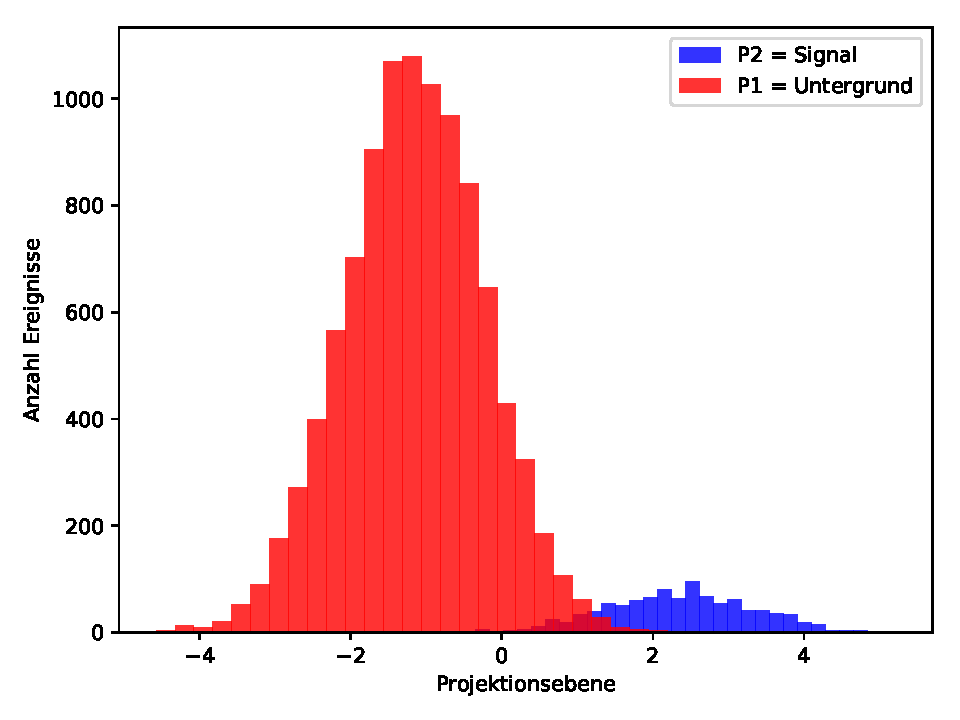
\includegraphics[scale=0.7]{Aufgabe12/Projektionen2.pdf}
  \caption{Eindimensionale Verteilung mit P2.}
  \label{abb:5}
\end{figure}

Die Effizienz und die Reinheit sind in Abbildung \ref{abb:6} zu sehen.
\begin{figure}
  \centering
  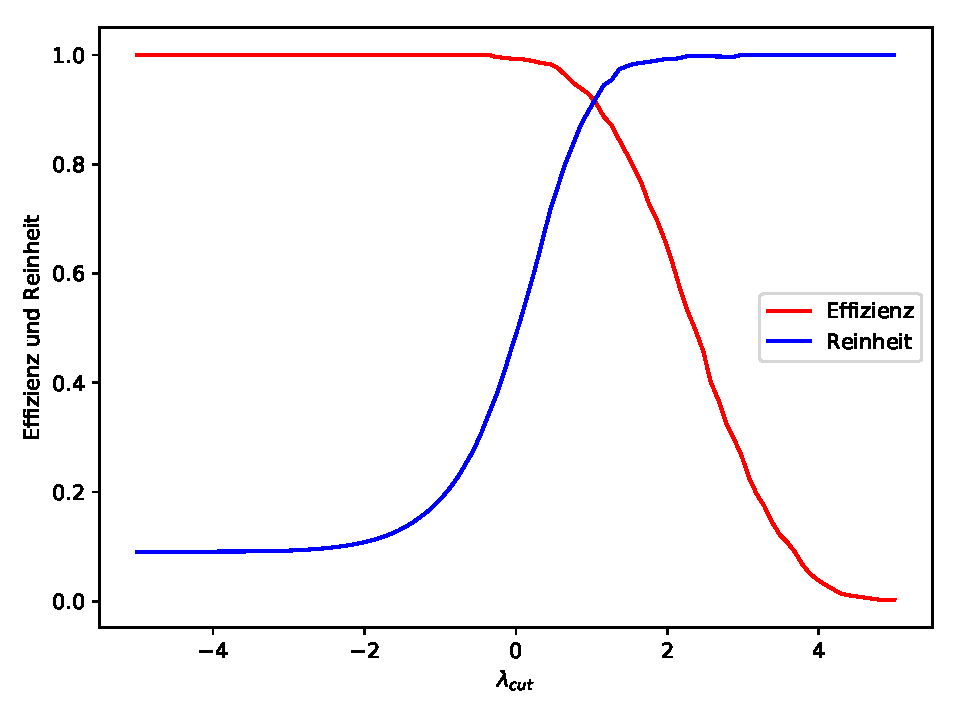
\includegraphics[scale=0.7]{Aufgabe12/EffizienzReinheit2.pdf}
  \caption{Effizienz und Reinheit der zweiten Verteilung.}
  \label{abb:6}
\end{figure}

Das Verhätnis $S/B$ in Abhängigkeit von der Cut-Stelle ist in Abbildung \ref{abb:7} dargestellt.
Das Maximum liegt bei:
\begin{equation*}
  \lambda_{\symup{cut,Verhältnis2}} \approx 2,27
\end{equation*}
\begin{figure}
  \centering
  \includegraphics[scale=0.7]{Aufgabe12/Verhältnis2.pdf}
  \caption{Verhältnis in Abhängigkeit der Cut-Stelle der zweiten Verteilung.}
  \label{abb:7}
\end{figure}

Die Signifikanzin Abhängigkeit von der Cut-Stelle ist in Abbildung \ref{abb:8} dargestellt.
Das Maximum liegt bei:
\begin{equation*}
  \lambda_{\symup{cut,Signifikanz2}} \approx 1,06
\end{equation*}
\begin{figure}
  \centering
  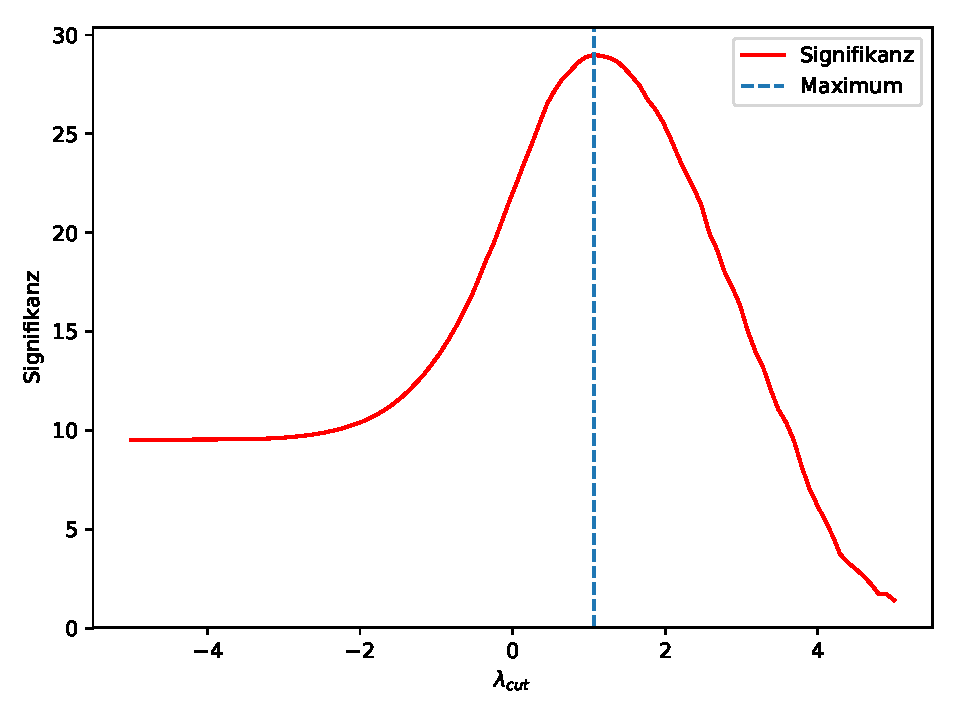
\includegraphics[scale=0.7]{Aufgabe12/Signifikanz2.pdf}
  \caption{Signifikanz in Abhängigkeit der Cut-Stelle der zweiten Verteilung.}
  \label{abb:8}
\end{figure}

Die Trennung funktioniert für kleinere oder gleichgroße Untergründe, im Bezug auf
das Signal, besser. Dies ist an den Maxima der Signifikanzkurve zu erkennen, da
das Maximum der ersten Verteilung deutlich höher liegt, als die der zweiten.

%\paragraph{Aufgabe 4}

\subparagraph{a)}

$P\left(W_\text{rot}+W_\text{blau}=9\right) \: = \: \SI{11,11}{\%}$

\subparagraph{b)}

$P\left(W_\text{rot}+W_\text{blau} \geq 9\right) \: = \: \SI{27,78}{\%}$

\subparagraph{c)}

$P\left(W_\text{rot}=4, W_\text{blau}=5\right \vee W_\text{rot}=5, W_\text{blau}=4) \: \geq \: \SI{5,56}{\%}$

\subparagraph{d)}

$P\left(W_\text{rot}=4, W_\text{blau}=5\right) \: \geq \: \SI{2,78}{\%}$

\subparagraph{e)}

$P\left(W_\text{rot}+W_\text{blau}=9 | W_\text{rot}=4\right) \: = \: \SI{16,67}{\%}$

\subparagraph{f)}

$P\left(W_\text{rot}+W_\text{blau} \geq 9 | W_\text{rot}=4\right) \: = \: \SI{33,33}{\%}$

\subparagraph{g)}

$P\left(W_\text{rot}=4, W_\text{blau}=5\right) \: \geq \: \SI{16,67}{\%}$

%\printbibliography{}


\end{document}
